\documentclass{article}
\usepackage[utf8]{inputenc}

\title{Command Center Information}
\date{February 2020}

\usepackage{natbib}
\usepackage{graphicx}

\begin{document}

\maketitle

\section{Introduction}
This is a prototype of a command center application/system. It logs sensor data from an external device, which is sent to the cloud and which can then be both read from a client application and stored as raw data on a database. The raw data can then be downloaded and postprocessed as seen fit.
The system consists of several different parts.
\begin{itemize}
\item Command Center Client
\end{itemize}
\begin{itemize}
\item Command Center Raspberry Pi Server
\item 	MQTT server in cloud
\item 	Different kinds of external equipment (Sensors, cameras etc.)
\item 	Kongsberg IMU and Seanav
\item 	Laptop for transmitting IMU and Seanav data
\end{itemize}



\begin{figure}[h!]
\centering
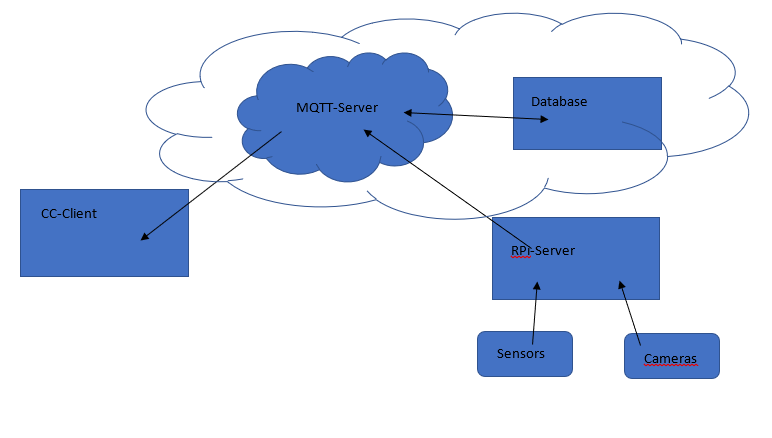
\includegraphics[scale=0.3]{Img/Image1}
\caption{Overview}
\label{fig:universe}
\end{figure}

\section{Client}
The client is what would be the command center, for a user. This is where one can monitor all the sensor data, camera stream, and see positional data on a map for example.
Currently there is only a one-way communication here, whereas the client only reads data coming from the cloud and displays them.
This is currently written as a C\# WPF desktop application. This means that the client must run on a Windows computer. The client can easily be re-written in any other language and framework to caters one’s specific use.

\section{RPi Server}
The Raspberry Pi is the main external device that must sit on the vessel in order to capture data and send it to the cloud. The RPi has internal sensors for measuring temperature, pressure, rotation and accelerations. These sensors are good for testing and prototyping but might not be the most accurate values. So, for proper readings, other sensors should be attached and used. One point is only that there is a limitation on how many sensors can be connected in terms of how much power they draw, since the Raspberry does not have that much power to give out to external sensors. Must be investigated more, where the limitations are.
If more and more sophisticated sensors are to be used, one might consider buying more RPi’s and use them together, or just swap out the whole function of the RPi by a laptop computer.

\section{MQTT Server}
The protocol used to exchange information between all the parts in the system, is called MQTT.
http://mqtt.org/
This is a message-based protocol, where one can publish and subscribe to messages with a specific topic. In this case, the client would be subscribed to a topic called “temperature” towards the server in the cloud, and when the RPi publishes towards this topic, the client will receive it. This is a very simple and easy system to work with, which makes the creation of a new client quite easy.
For monitoring of the messages flowing through the MQTT server, an application like MQTT.fx can be used. https://mqttfx.jensd.de/
This server will run in the cloud, for example in Microsoft Azure as a virtual machine running Ubuntu.
This virtual machine needs to be set-up, and MQTT has to be installed. Running a virtual machine in the cloud will have some costs.

\section{Database}
The database is a NoSQL database, also in the cloud. This can be a separate machine, or database solution, but for simplicity we can just install a CouchDB database on the same virtual machine as the MQTT server is running.
The database could also just be installed on the Raspberry Pi and store all the data locally there if there is too much trouble creating a database in the cloud. This could also be a good backup solution for when running a sea trial.
If the database is in the cloud, then it will have a database client which also listens to the MQTT server and stores all the data it is listening to in the database.
Information on how to operate a CouchDB can be found here: https://docs.couchdb.org/en/stable/

\section{Sensors}
Several different sensors can be used. The most interesting one might be those who provides positional data, like coordinates, speed, accelerations and orientations.
For the to be connected to the RPi, it is the easiest to use sensors that have USB.
There are possibilities to use other kinds of sensors too, but that might require some additional parts to the RPi. Another limitation as mentioned earlier is the power capabilities, which one must consider. There should also be a USH hub, which can be used to get more usb ports for more sensors.
The sensors we currently have:
\begin{itemize}
\item 	RPi sensor HAT
\begin{itemize}
\item	Provides orientation, acceleration, temperature, pressure
\end{itemize}
\item 	2 IR temperature sensors
\begin{itemize}
\item 	Provides temperature at what they’re pointed at
\end{itemize}
\item 	HD Camera
\begin{itemize}
\item 	This takes a lot of power. This camera together with another USB camera was too much, and it didn’t work.
\end{itemize}
\item 	RPi Camera
\item 	USB GPS
\begin{itemize}
\item 	Impossible to establish GPS contact with this one inside buildings. Needs to have clear sight to sky.
\end{itemize}
\item 	Kongsberg SEANAV (OBS: Rented, needs to be returned at end of lease)
\begin{itemize}
\item 	GPS, Speed, etc.
\item 	See user manual for capabilities.
\item 	Needs to be set-up correctly in terms of network settings etc. to communicate with Pi.
\end{itemize}
\item 	Kongsberg IMU (OBS: Rented, needs to be returned at end of lease)
\begin{itemize}
\item 	Accelerations, rotations, orientations.
\item 	See user manual for capabilities.
\item 	Needs to be set-up correctly in terms of network settings etc. to communicate with Pi.
\end{itemize}
\end{itemize}

So, the most interesting sensors here are definitively the two from Kongsberg.
They are the ones providing the useful and interesting information here. But they’re also the hardest to set-up, and I do not remember everything on the fly here, without trying them.


\section{Client Installation}
\subsubsection{Workstation set-up}
The current client needs Windows to run. As far as I know, the workstation to be used for this currently has a Linux set-up.
The first step is then to install Virtual Box on the Linux computer. (https://www.virtualbox.org/)
You then need an image of a Windows installation, which has to be obtained from somewhere.
It might be best to ask IT at UiT to help with getting Windows installed as a virtual machine on the computer. When this project was started, it was assumed that this computer would be running Windows. So, another project could be to re-write the client in something that is supported cross platforms. Like in Python or C++. Could be a student project.
\subsection{Client Environment}
Assuming we have a Windows computer now, then we need to install Visual Studio. (https://visualstudio.microsoft.com/)
This is what we can use to build the project and modify it however we want.
We could also just run the client from here.
We also must install Git, which is a source control system. (https://git-scm.com/)
After we have git, we need to pull the project from GitHub. (https://github.com/steinmal/command-center-client). To lean how to pull a project, and use git, look up some tutorials online.
It should now be possible to open the project inside Visual Studio.
Update all Nuget Packages and try to build the project.
For the client to be working with the server you will be setting up, you need to alter the ip-adress that is used in the source code.

\section{RPi Server Installation}
\subsection{Connection to internet}
The RPi needs to be connected to the internet, for testing purposes this could be done over WIFI.
You then need to connect the RPi to a screen, mouse and keyboard. Then turn it on and connect to WIFI as you usually would to on a computer.
NB: If you however are going to communicate with the Kongsberg equipment, then you must get internet via ethernet cable in to the RPi. The set-up used in this case, would be Mobilt bredbånd using a router that has three ethernet exits. Where the router gets internet via 4G, and one ethernet cable goes to each of the Kongsberg equipment and one cable goes to the RPi.

\subsection{Connection to RPi}
After the RPi has been connected to the internet, it should get an IPv4 address which will be displayed on the small LED screen. You can then SSH to the RPi, and communicate with it through SSH. This can either be done with the ssh command from a linux computer or if using Windows a client like PuTTy. (https://www.putty.org/)
Where you connect to the Pi with the address showing on the LED display and port 22.
If successful you’ll be prompted for a username and password, which is currently:
u: pi
p: commandcenter

Now you can write XXXXXXXX to run the server, which will start reading data and sending them. 
To abort the running server, you’ll have to press CTRL+Z twice.

\section{Cloud Server Installation}
As mentioned earlier, one need to acquire a virtual machine with Ubuntu in some cloud service. For example, in Microsoft Azure. There should exist guides for this online.
On this VM, one needs to install the MQTT server. This should be done as described her: 
https://appcodelabs.com/introduction-to-iot-build-an-mqtt-server-using-raspberry-pi
The guide is for a RPi, but it’s the same for Ubuntu.
An important thing about running servers on virtual machines in Azure, is that you must explicitly open ports on the VM in the Azure dashboard, so it’s possible to access it from the outside.
For MQTT servers the port that needs to be opened is 1883.
For SSH access, it’s port 22.
For CouchDB it’s 5984.
To install couch, follow the instructions on https://docs.couchdb.org/en/stable/install/index.html

\section{SSH Tunneling}
It proved to be difficult to open the ports on a Mobilt Bredbånd router, which means it’s not possible to connect from the outside to the Pi. If you want SSH access to the Pi from outside it’s network, you’ll have to set it up with SSH tunneling towards the VM in the cloud, and remember to open the appropriate ports. Online guides on this should exist. But might not be a necessary feature.

\section{SEANAV and IMU}
Refer to their user manuals on how to set-them up.
They should work well with just connecting them. Important points are that the IP addresses must be correct. Either the SEANAV or the IMU needs to be in a specific IP range, so then the whole system needs to be in this range too.
To enter the settings of these devices, connect them to a laptop which has the set-up software installed. Refer to manuals.

\section{RPi Sense Hat}
This sensor works straight out of the box. Refer to the code or examples online to see how to access the values.

\section{IR Temperature Sensors}
These can be a little tricky to get to work without some set-up. Some Linux set-up is needed for them to be recognized automatically regardless of which usb port is used. The code needs to point to the correct port.

\section{USB GPS}
I think this should work out of the box,
but it’s really hard to test because it’s so bad at getting a signal with any obstructions.

\section{Final Notes}
It should be considered to transfer the projects from GitHub to UiT’s own source control system.

\end{document}
